%
% $RCSfile: peer_node.tex,v $
%
% Copyright (C) 2002-2008. Christian Heller.
%
% Permission is granted to copy, distribute and/or modify this document
% under the terms of the GNU Free Documentation License, Version 1.1 or
% any later version published by the Free Software Foundation; with no
% Invariant Sections, with no Front-Cover Texts and with no Back-Cover
% Texts. A copy of the license is included in the section entitled
% "GNU Free Documentation License".
%
% http://www.cybop.net
% - Cybernetics Oriented Programming -
%
% http://www.resmedicinae.org
% - Information in Medicine -
%
% Version: $Revision: 1.1 $ $Date: 2008-08-19 20:41:08 $ $Author: christian $
% Authors: Christian Heller <christian.heller@tuxtax.de>
%

\section{Peer Node}
\label{peer_node_heading}
\index{Peer Node}
\index{Distributed System}
\index{Distributed Computing Environment}
\index{DCE}
\index{c/s}
\index{Peer-to-Peer}
\index{P2P}
\index{Client}
\index{Server}
\index{Freenet}
\index{Gnutella}
\index{BitTorrent}
\index{eDonkey}
\index{FastTrack}
\index{Napster}

Tanenbaum and Steen \cite{tanenbaum2002} define a \emph{Distributed System} as
\textit{a collection of independent computers that appear to its users as a
single coherent system}. With \emph{System} referring to a process rather than
only hardware, as defined in section \ref{process_heading}, it seems appropriate
to rephrase and use this for the definition of a general
\emph{Distributed Computing Environment} (DCE):

\begin{quote}
    A distributed computing environment consists of at least two systems that
    work together over a network but run on independent computer hardware (nodes).
\end{quote}

\begin{figure}[ht]
    \begin{center}
        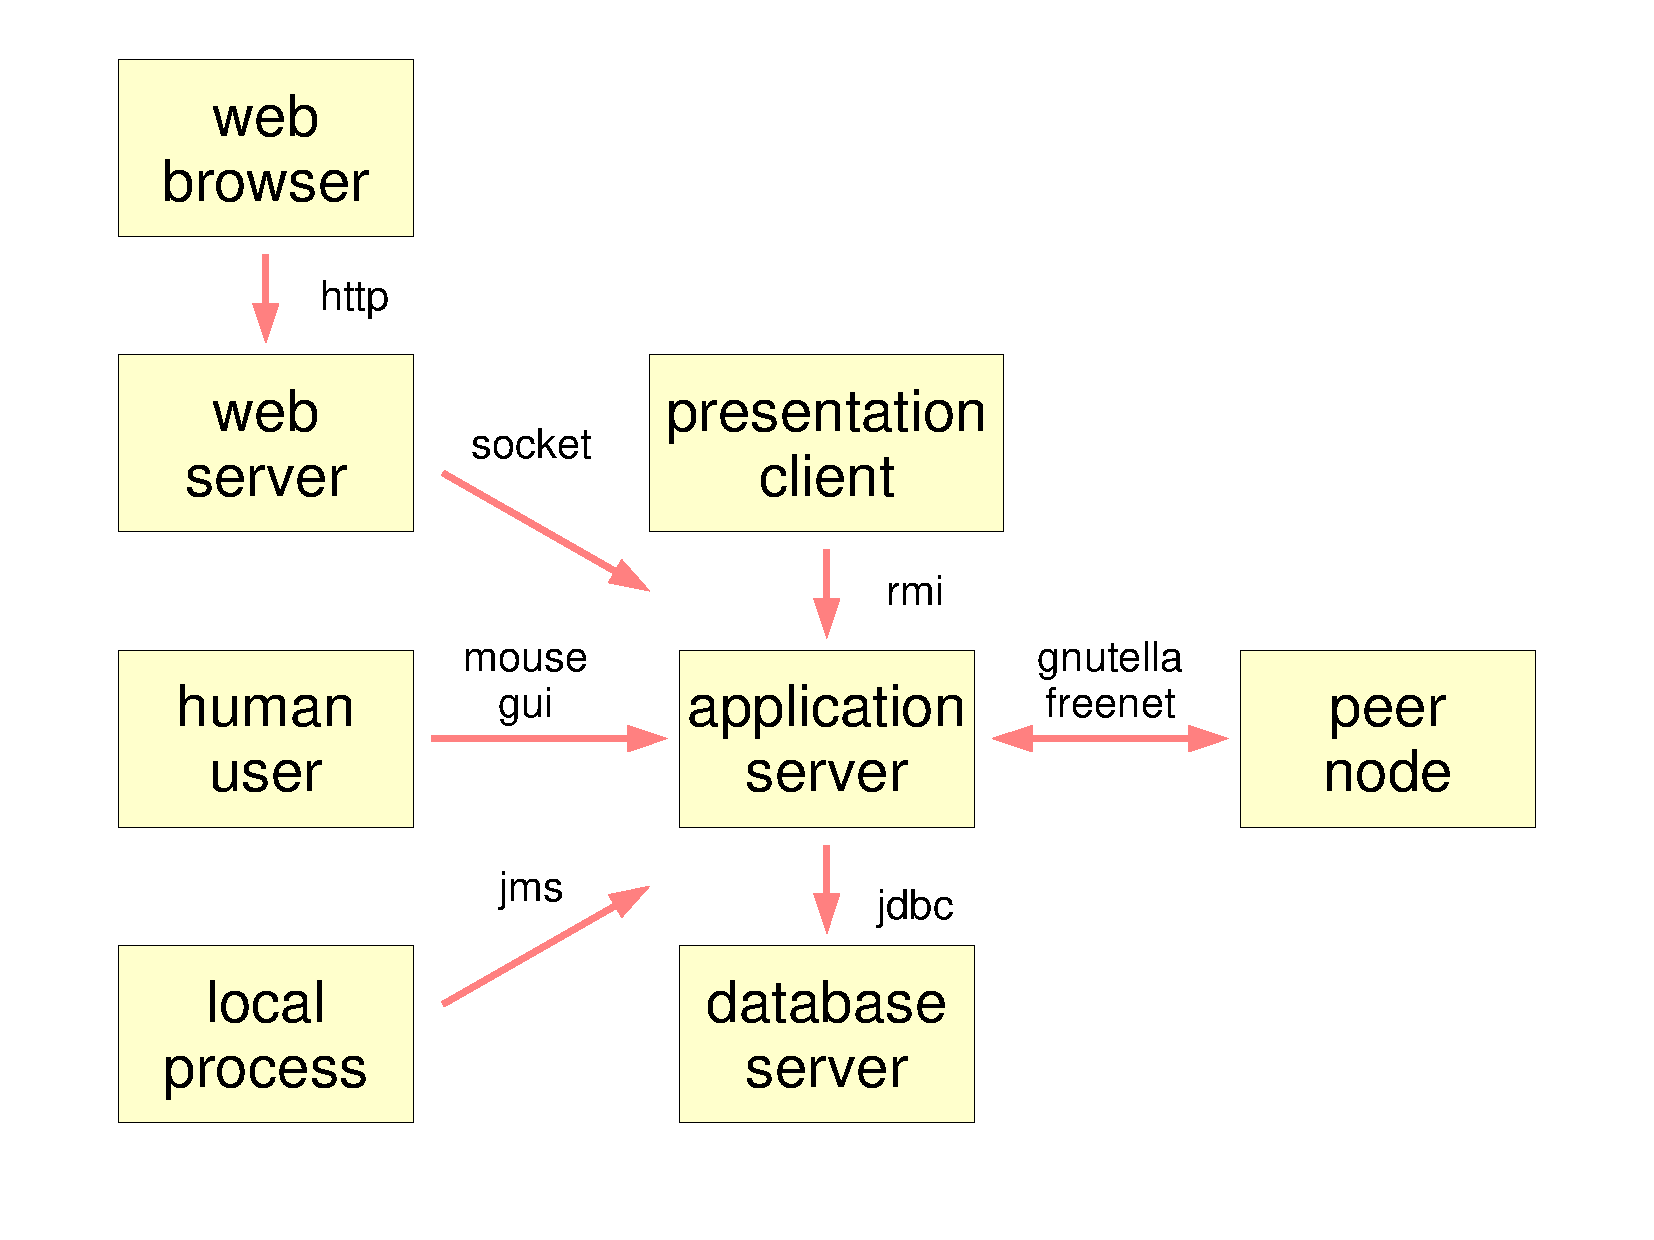
\includegraphics[scale=0.3,angle=-90]{graphic/peer.pdf}
        \caption{Peer-to-Peer Node Communication}
        \label{peer_figure}
    \end{center}
\end{figure}

Besides the previously mentioned client/ server (c/s) environments, so-called
\emph{Peer-to-Peer} (P2P) computer networks latterly became popular. In them,
nodes do not have just one role, but act as client and server at the same time
(figure \ref{peer_figure}), thus sharing their computing power and bandwidth.
Common P2P protocols are: \emph{Freenet}, \emph{Gnutella2}, \emph{BitTorrent},
\emph{eDonkey}, \emph{FastTrack} or \emph{Napster} \cite{wikipedia}. Many more
exist.

Just like nodes in a P2P network, human beings are capable of communicating
both ways, taking the role of a client or server. The organs that are needed to
do so are put into comparison with the corresponding devices of a computer
system, in chapter \ref{state_and_logic_heading}.
